\chapter{Background}

\label{chap:background}

\section{Recommender Systems}

\label{sec:background_recommend}

A recommender system uses data to suggest potentially interesting items to users, including items that a user may not have heard of before \cite{LU20121}. Items refer to products, services or other objects that can be evaluated. 

The recommendations produced by a recommender system can be personalized recommendations and may differ from user to user \cite{LU20121}. These recommendations can be represented by scores on unrated items. A higher score indicates that an item could be preferred over an item with a lower score.

In the following we define a target user and try to find a recommendation for set user.

We now classify recommender systems like \cite{LU20121, itemColFiltRecom} into:

\begin{itemize}
    \item \textbf{Content-based Filtering}: recommendations are generated through item characteristics and user ratings
    \item \textbf{Collaborative Filtering}: recommendations are based only on previously made ratings by the target user and all other users. 
\end{itemize}

In this paper, we only use algorithms that are in the Collaborative Filtering domain. 

The Collaborative Filtering approach can be further divided into:

\begin{itemize}
    \item User (or memory) based collaborative filtering \cite{itemColFiltRecom, LU20121}: This approach uses all ratings from all users and compares the target user's ratings to all other ratings to find users similar to the target user.\cite{itemColFiltRecom}. 

Our assumption is that if users can come to an agreement on one item, then they can also come to an agreement on other items \cite{LU20121}.
    \item Item (or modeling) based collaborative filtering \cite{itemColFiltRecom, LU20121}: This approach compares only the ratings of the target item with the ratings of other items. This allows a similarity between items to be found \cite{itemColFiltRecom}.
\end{itemize}

A representative rating would be, for example, the 5 star rating system used by Amazon and other stores \cite{LU20121, miningOfMassiveDatasets}. On this basis, a user can evaluate and rate a consumed item. Another rating system could be an implicit system, where consuming an item generates a rating \cite{miningOfMassiveDatasets}. In this case, the rating wouldn't reflect whether a user actually liked the item.


\subsection{Similarity}

In this section we will mainly talk about user-based collaborative filtering, the same applies to item-based collaborative filtering. We will explicitly address the differences.

An important task in recommending items to a target user is to determine how similar the target user is to other users. To get a better understanding of how similarity between users can work, similarity is treated as a distance: the closer users are to each other, the more similar they are. We consider the following algorithms to calculate such a distance:

\begin{itemize}
    \item  \textbf{Euclidean distance}: This algorithm makes use of the euclidean distance between two vectors \cite{miningOfMassiveDatasets}. In this case, we take all of a user's ratings as a vector in an n-dimensional space, where n is the number of items. We can then calculate the distance to another vector, or in this case another user. One problem with this algorithm is how to deal with unrated items, since we can't compare two points with different dimensions. In this case we simply set the unvalued points to zero, so that the two points have the same dimensions again.

    \newpage

    \begin{figure}[h!]
    \centering
    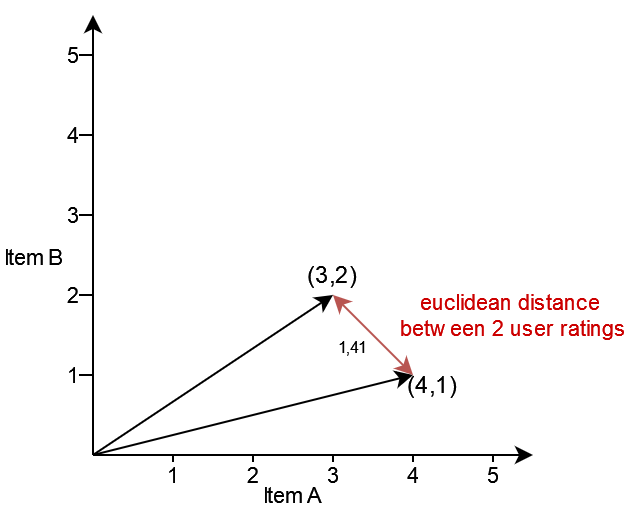
\includegraphics[width=\textwidth/2]{images/recommend/euclidian_distance_vis.drawio.png}
    \caption{\label{fig:recommend_euclid}Euclidean distance with two items and two user ratings}
    \end{figure}

    \item \textbf{Cosine distance}: This algorithm has a similar approach to the Euclidean distance, but with the cosine distance we compare the angle of the direction of the vectors \cite{miningOfMassiveDatasets}. In this case, we don't take into account the length of the vector, which can make the recommendation imprecise. This doesn't mean that the recommendation is worse than, for example, the Euclidean distance.

    \begin{figure}[h!]
    \centering
    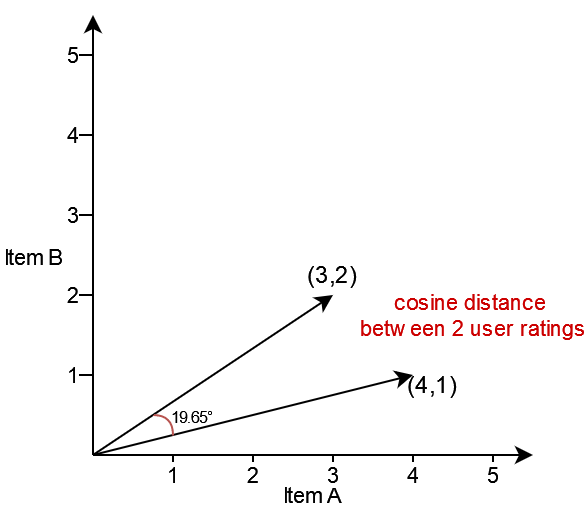
\includegraphics[width=\textwidth/2]{images/recommend/cosine_distance_vis.drawio.png}
    \caption{\label{fig:recommend_euclid}Cosine distance wit two items and two user ratings}
    \end{figure}

    \item \textbf{Pearson distance (Adjusted Cosine for Item based Collaborative Filtering)}: With Pearson, we use the same approach as with cosine distance, but with Pearson we normalise the ratings of all users before calculating a distance. Normalisation avoids the problem of favouring ratings from users with similar user biases to the target user \cite{miningOfMassiveDatasets}. A user bias occurs when a user rates items overwhelmingly positively or negatively. 

With the adjusted cosine (in item-based filtering domain), we don't want to normalise the item ratings because the item bias is the recommendation. Instead, we also normalise the user ratings as we do with the Pearson distance and then use the adjusted ratings for the cosine distance \cite{miningOfMassiveDatasets}.

\end{itemize}

Using these similarity measures, we can now select the most similar neighbours.

\subsection{Recommend an item}

Once we have found the k nearest neighbours, we can calculate an estimated rating of an unrated item for the target user. 

With user-based collaborative filtering, we look at the ratings of the k nearest users of an item that the target user hasn't rated. The average of these ratings can then be used as an indicator of whether or not the target user would like the item.

\begin{equation}
M_{u} = \frac{\sum_{i=1}^{k}{rating_i}}{k}
\label{mean}
\end{equation}

We can also take the weighted average to get a potentially more accurate recommendation:

\begin{equation}
M_{w} = \frac{\sum_{i=1}^{k}{rating_i * similarity_i}}{\sum_{i=1}^{k}{similarity_i}}
\label{weightedMean}
\end{equation}


This estimate reflects a possible rating of the target user. It also has the advantage that it can be used to test the recommendation system by trying to guess a rating that the user has already given and checking how much the estimated rating differs from the actual rating \cite{miningOfMassiveDatasets}. 

\section{Business Process Modelling Notations}

\label{sec:background_bpmn}

Business process modelling is an approach of describing the logical process in a business environment with a desired outcome \cite{bpm_review_framework}. Although many organisations use whiteboards or Microsoft Office to model processes, there is a trend towards using formal business process modelling notations (BPMN) \cite{ebpma-tec-standards, bpm_review_framework}. The benefits of formal BPMN are precision and reliability, so that everyone involved doesn't have to guess what different components of a notation mean \cite{ebpma-tec-standards}.

There are many BPMNs to choose from, \cite{bpm_review_framework} categorises them into different techniques:

\begin{itemize}
    
    \item \textbf{Flow Chart technique}: a simple, flexible and graphical approach to process modelling. Because of it's flexible design, it can also be used for logical sequences or as an organisation chart. 

    \begin{figure}[h]
    \centering
    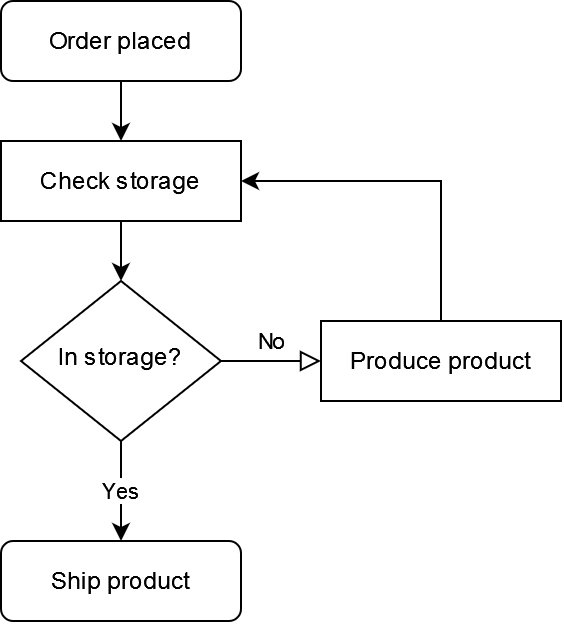
\includegraphics[width=\textwidth/3]{images/BPMN/flow_sample.drawio.png}
    \caption{\label{fig:bpmn_flow_chart}Flow Chart}
    \end{figure}

    
    \item \textbf{Data Flow diagrams}: a diagramming that visualises the flow of data or information between locations. It's often used between analysts and users because it's easy to understand and the connection points can be easily split to get more information.

    \begin{figure}[h]
    \centering
    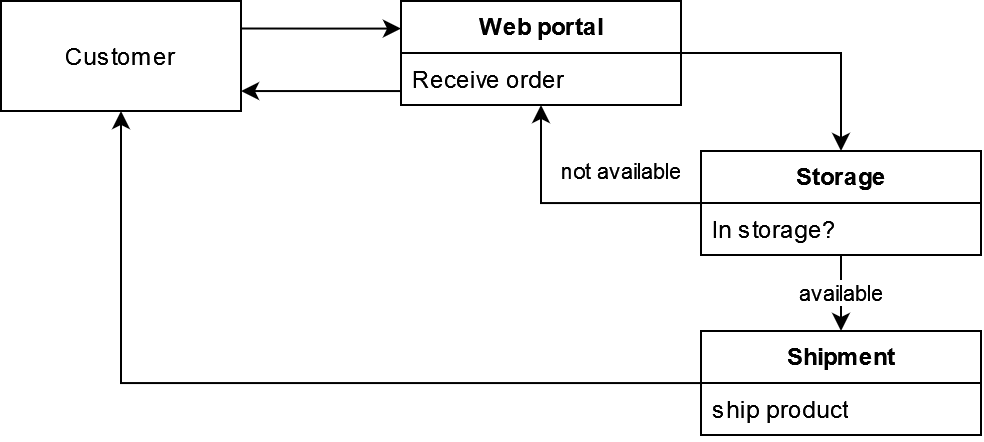
\includegraphics[width=\textwidth/3]{images/BPMN/dataflow_sample.drawio.png}
    \caption{\label{fig:bpmn_dataflow_diagram}Data Flow Diagram}
    \end{figure}

\newpage
    
    \item \textbf{Role activity diagrams}: a diagram that visualises a process from the perspective of a single role. Roles are abstract and describe a desired behaviour like an object in an object-oriented environment.
    
    \item \textbf{Role interaction diagrams}: A matrix-like diagram that describes a process through activities or connections between roles. Activities are actions a user can take, such as ordering a product. It's not as flexible as a flow chart, but still easy to understand.

    \begin{figure}[h]
    \centering
    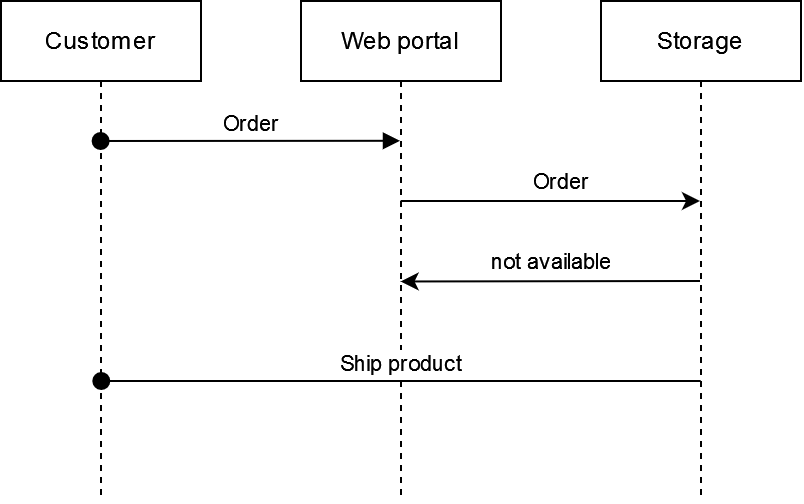
\includegraphics[width=\textwidth/2]{images/BPMN/role_int_sample.drawio.png}
    \caption{\label{fig:bpmn_RID_chart}Role interaction diagram}
    \end{figure}
    
    \item \textbf{Gantt Chart}: a matrix that describes a process through activities and time periods. The matrix can also includes names/actors or skill levels that perform an activity.

    \begin{figure}[h]
    \centering
    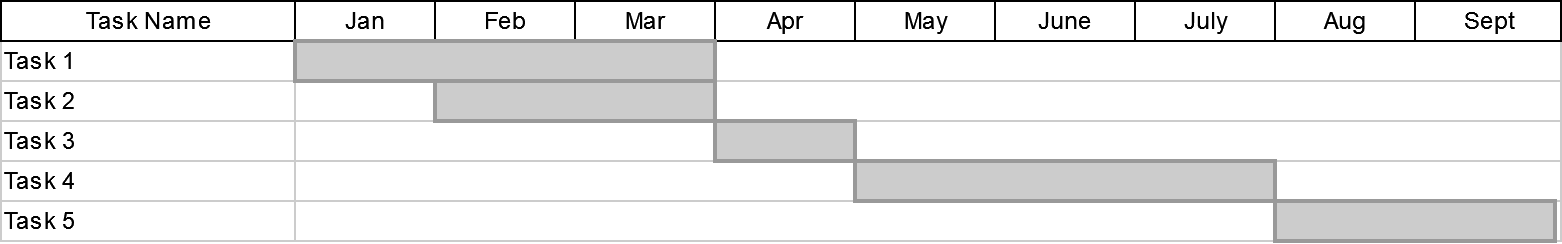
\includegraphics[width=\textwidth/2]{images/BPMN/Gnatt_sample.drawio.png}
    \caption{\label{fig:bpmn_gnatt_chart}Gantt Chart}
    \end{figure}
    
    \item \textbf{Integrated Definition for Function Modelling (IDEF)}: is a family of methods for modelling processes. The most useful are IDEF0 and IDEF3 for business process modelling and use activities that can also be represented as a sequence.

    \begin{figure}[h]
    \centering
    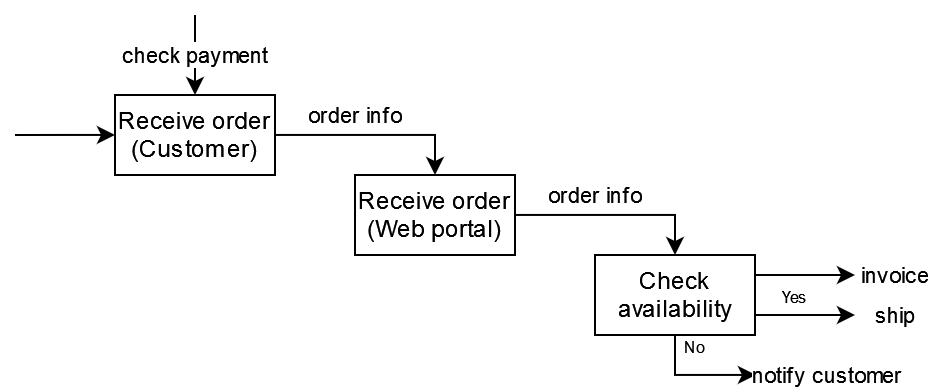
\includegraphics[width=\textwidth/2]{images/BPMN/idef_sample.drawio.png}
    \caption{\label{fig:bpmn_IDEF_diagram}IDEF0 diagram}
    \end{figure}
    
    \item \textbf{Coloured Petri-net}: is a graphical language that is useful when working with many processes that communicate and synchronise. The model contains modules, which in turn contain places and connections between them.
    
    \item \textbf{Object oriented methods}: combines data structures and behaviour. This allows an object to represent an entity that has a function in the real world and to interact with other entities.

    \begin{figure}[h]
    \centering
    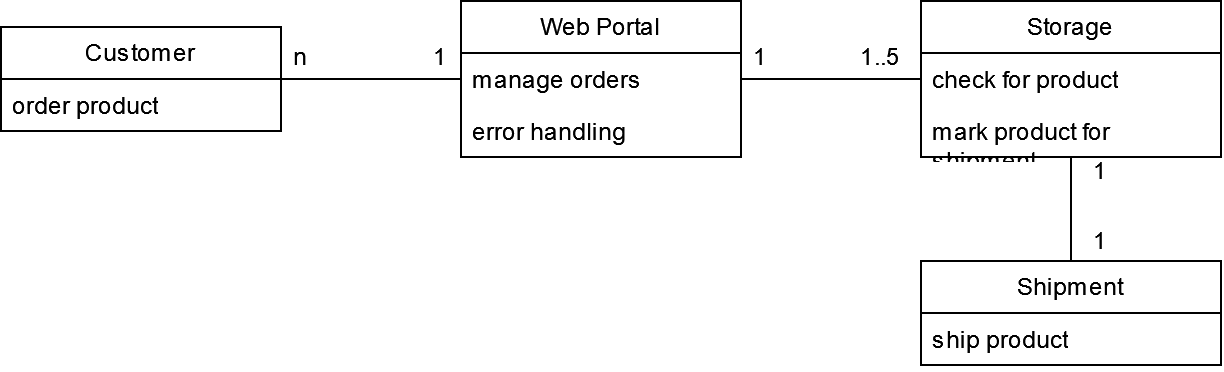
\includegraphics[width=\textwidth/2]{images/BPMN/uml_sample.drawio.png}
    \caption{\label{fig:bpmn_uml_diagram}UML diagram as a example of object oriented methods}
    \end{figure}
    
    \item \textbf{Workflow technique}: as the name suggests, data and information is passed from one node to another for further processing. Each node can take actions to achieve a common goal with other nodes. 
    
\end{itemize}

As we have seen, each technique has its advantages and its disadvantages.